\subsection{Beam Quality(Purity)}

We have several beam counters to identify beam particles event by event(see Fig. \ref{fig:Beamline}).
Beam includes $K^{+}$, $\pi^{+}$, $e^{+}$ and $p$ which have the momentum adjusted $\sim$800MeV/c.
We need to obtain $K^{+}$,$\pi^{+}$ and $p$ events and to reject $e^{+}$ events for analysis.
Fitch Cherenkov Counter is the differential-type detector which can seperate particles into $K^{+}$ and $\pi^{+}$ with differences of angle which cherenkov light emitted.
As shown in Fig. \ref{fig:FC_KPI}, the response of Fitch Cherenkov Counter are categorized into three, $K^{+}$ like, $\pi{+}$ or $e^{+}$ like and $p$ like.
Why $\pi^{+}$ like and $e^{+}$ like are same category is the velocities of both particles are very close.
Gas Cherenkov Counter is the threshold-type detector which can select $e^{+}$ because only $e^{+}$ can emitted cherenkov light in the gas of the detector.
Fig. \ref{fig:GC} shows the response of Gas Cherenkov Counter, and we define the events GC signal are above dashed line as $e^{+}$ events.
Tab. \ref{tb:Summary} shows whether the particles leave signals on each detector.\\

\begin{figure}[htbp]
  \centering
  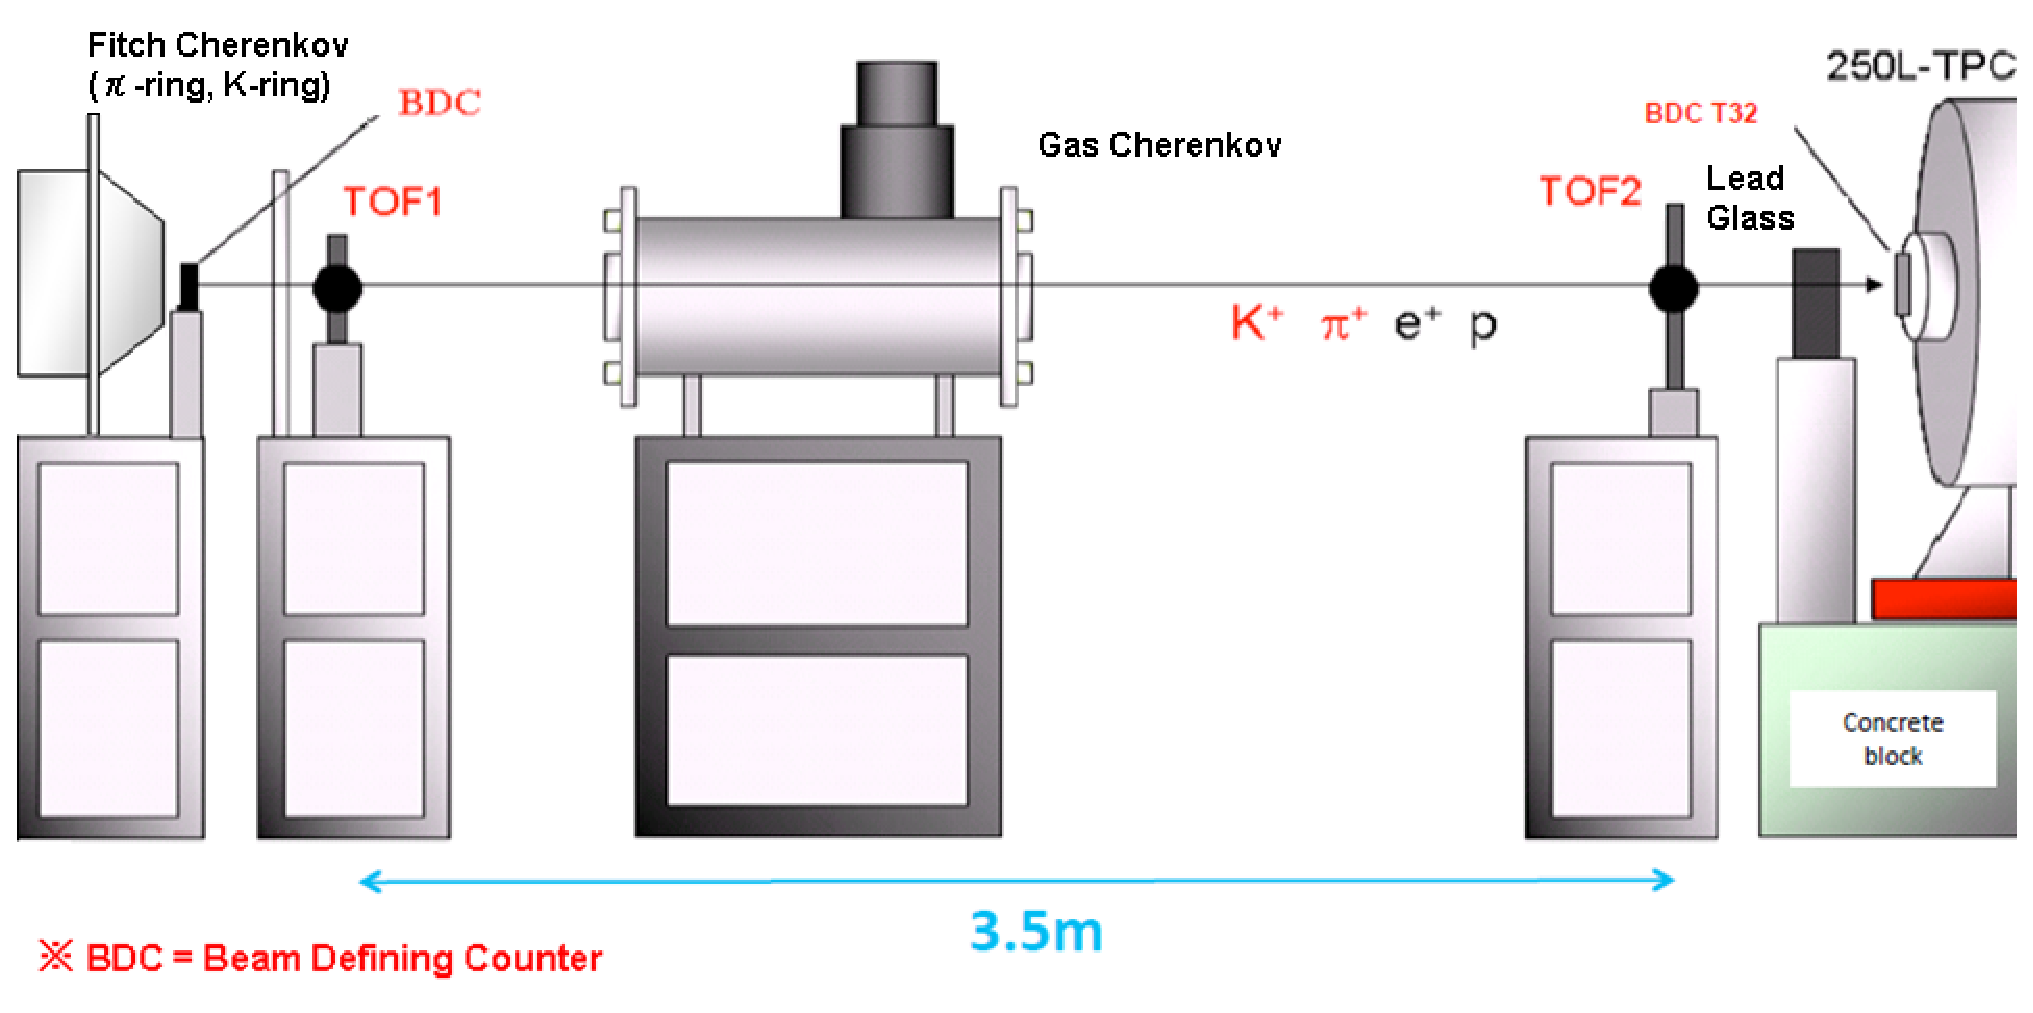
\includegraphics[width=10cm,clip]{fig/Beamline.eps}
  \caption{Instruments on K1.1BR Beam Line}
  \label{fig:Beamline}
\end{figure}

\begin{table}
  \centering
  \caption{Detector response}
  \begin{tabular}[htb]{c|cccc} \hline
    Particle  & FC(K) & FC($\pi$) & GC \\ \hline
    $\pi^{+}$ & x     & o         & x  \\
    $K^{+}$   & o     & x         & x  \\ 
    $p$       & x     & x         & x  \\ 
    $e^{+}$   & x     & o         & o  \\ \hline
  \end{tabular}
  \label{tb:Summary}
\end{table}

\begin{table}
  \centering
  \caption{Time of flight of each particle}
  \begin{tabular}[htb]{c|cccc}\hline
    particle & $e^{+}$ & $\pi^{+}$ & $K^{+}$ & $p$ \\ \hline
    Mass(MeV) & 0.511 & 139.57 & 493.68 & 938.27 \\
    Time of Flight($ns$) & 11.67 & 11.84 & 13.71 & 17.98 \\ \hline
  \end{tabular}
  \label{tb:TOF_expect}
\end{table}

As shown in Tab. \ref{tb:Summary}, we can seperate particles into above four particles by using the information of Fitch Cherenkov Counter and Gas Cherenkov Counter.
In addition, we can increase the purity of each particle by using the information of TOF Counter.
There are two TOF Counters which have $\sim$200 ps resolution 3.5m apart, 
and each particle is seperated with the difference of time of flight between them.
Table \ref{tb:TOF_expect} is calculated time of flight when each 800MeV/c particle passes two counters.
As shown Tab. \ref{tb:TOF_expect}, TOF Counter cannot seperate $e^{+}$ and $\pi^{+}$ because the difference of time of flight is too short for the TOF resolution.
Fig. \ref{fig:TOF} shows the response of TOF Counter, and they are categorized into three, $\pi{+}$ or $e^{+}$ events, $K^{+}$ events, $p$ events.
Herewith we can obtain high-purity samples of each particle by using the information of Fitch Cherenkov Counter, Gas Cherenkov Counter and TOF Counter.
We have obtained $K^{+}$ events by requiring the condition FC($K$) signal is above 2000 as trigger.
Fig. \ref{fig:TOF_cut} shows the response of TOF Counter after required the above condition.
Even though a few events which are defined as $K^{+}$ like events at Fitch Cherenkov Counter exude $\pi$ event region at TOF Counter,
we can reject those events by using this information and obtain $K^{+}$ samples of $\sim$100$\%$ purity.
Tab. \ref{tb:beam_component} shows particle fraction of samples used for analysis.(Total number of all four particles is 100)\\

\begin{figure}[htbp]
  \begin{tabular}{cc}
    \begin{minipage}{0.5\hsize}
      \centering
      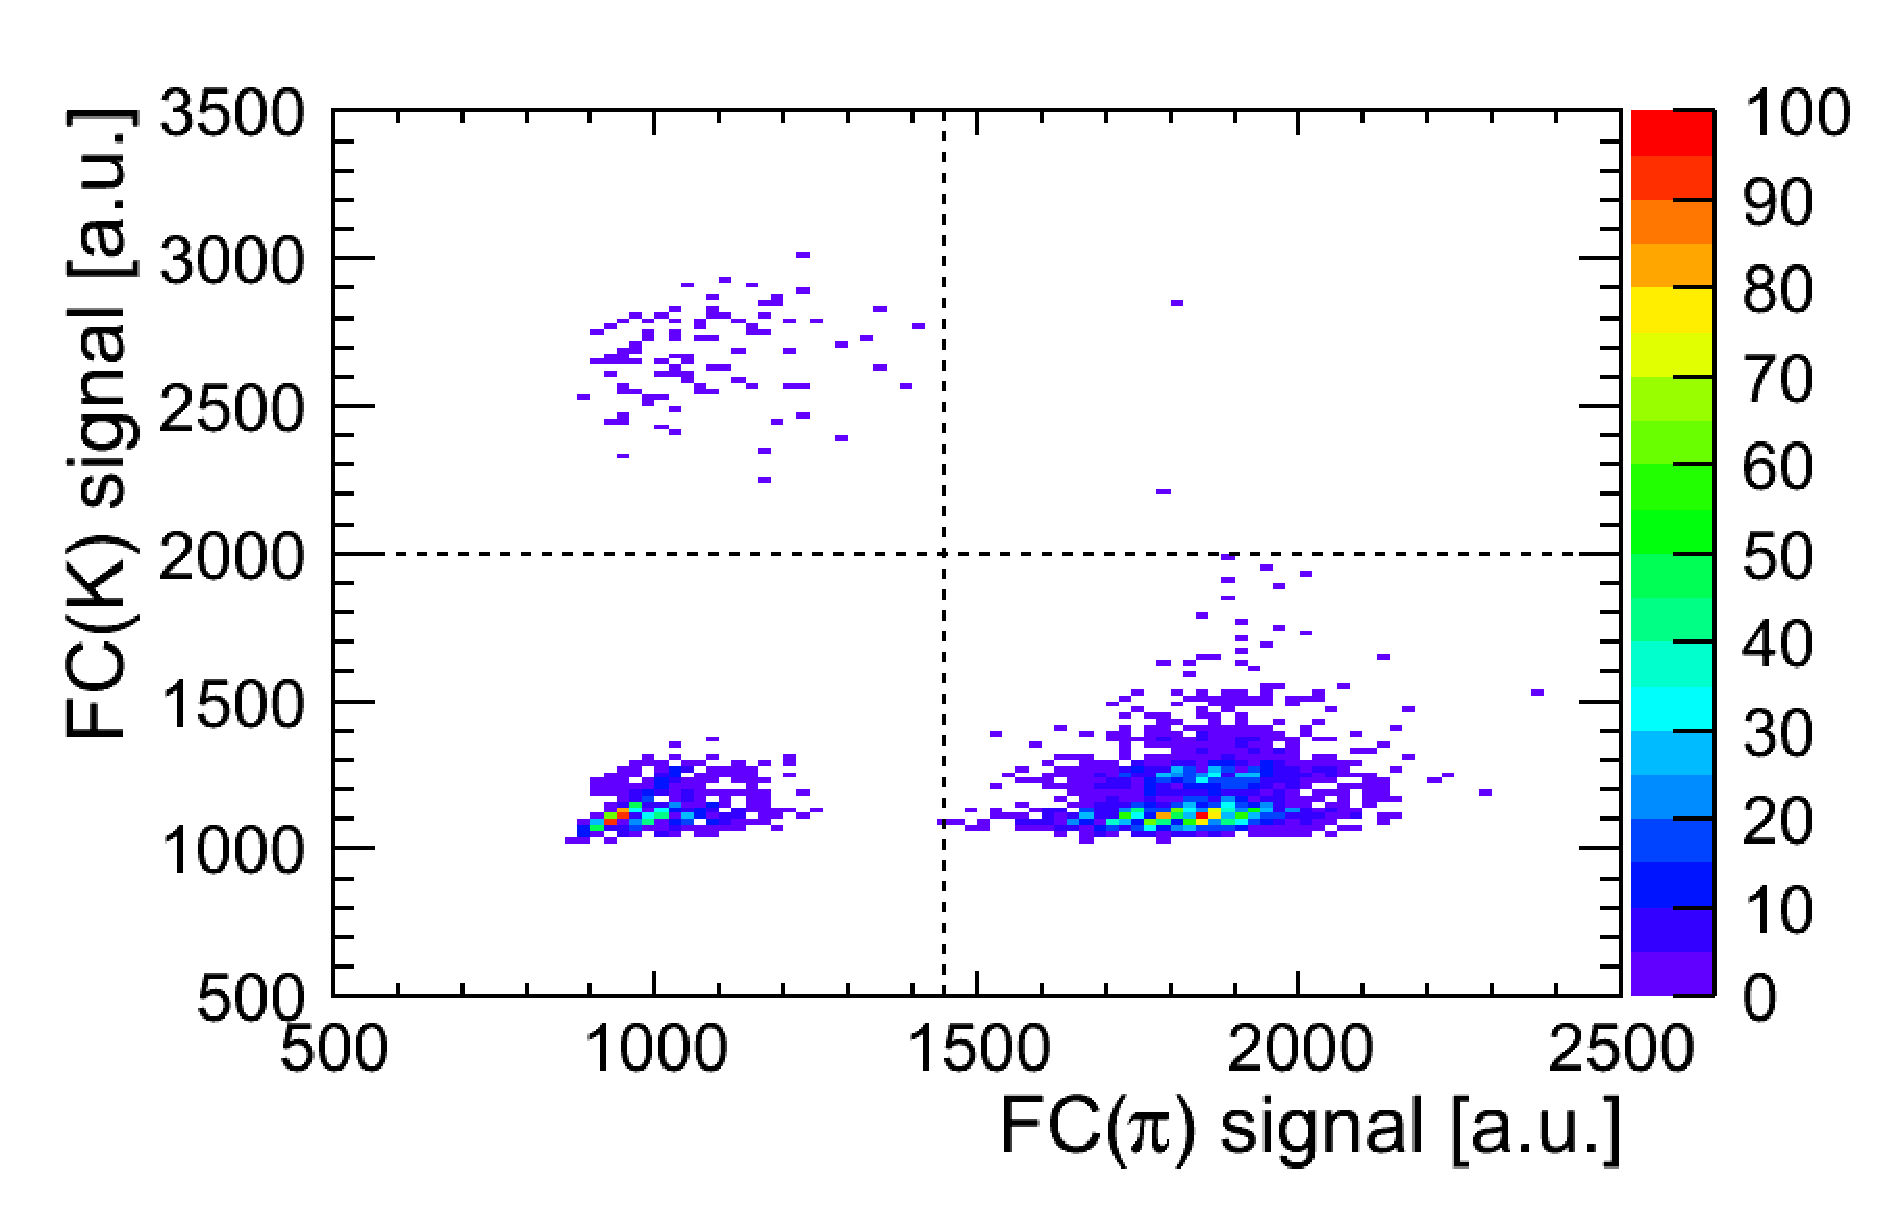
\includegraphics[width=6cm,clip]{fig/FC_KPI.eps}
      \caption{Fitch Cherenkov Counter}
      \label{fig:FC_KPI}
    \end{minipage}
    \begin{minipage}{0.5\hsize}
      \centering
      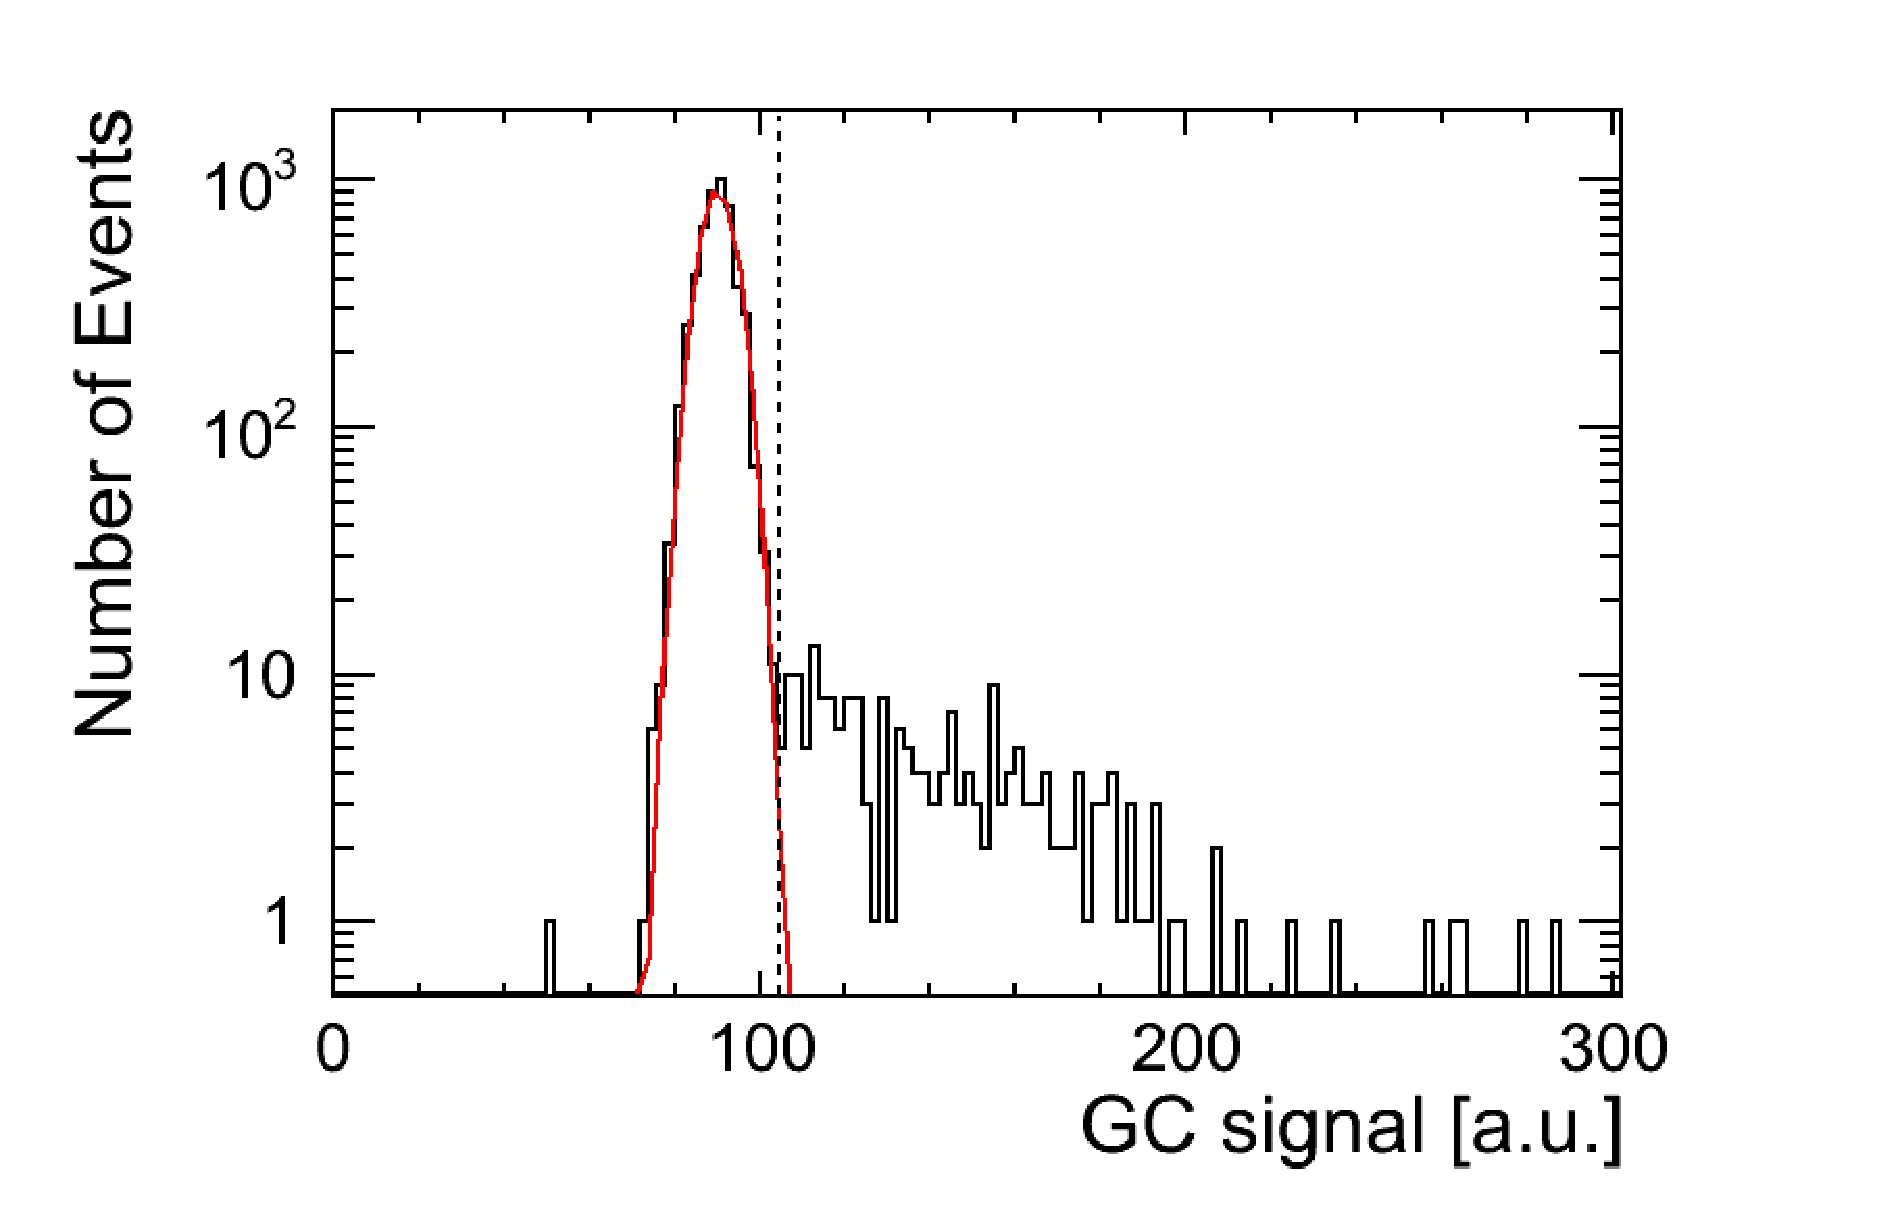
\includegraphics[width=6cm,clip]{fig/GC.eps}
      \caption{Gas Cherenkov Counter}
      \label{fig:GC}
    \end{minipage}
  \end{tabular}\\
  \begin{tabular}{cc}
    \begin{minipage}{0.5\hsize}
      \centering
      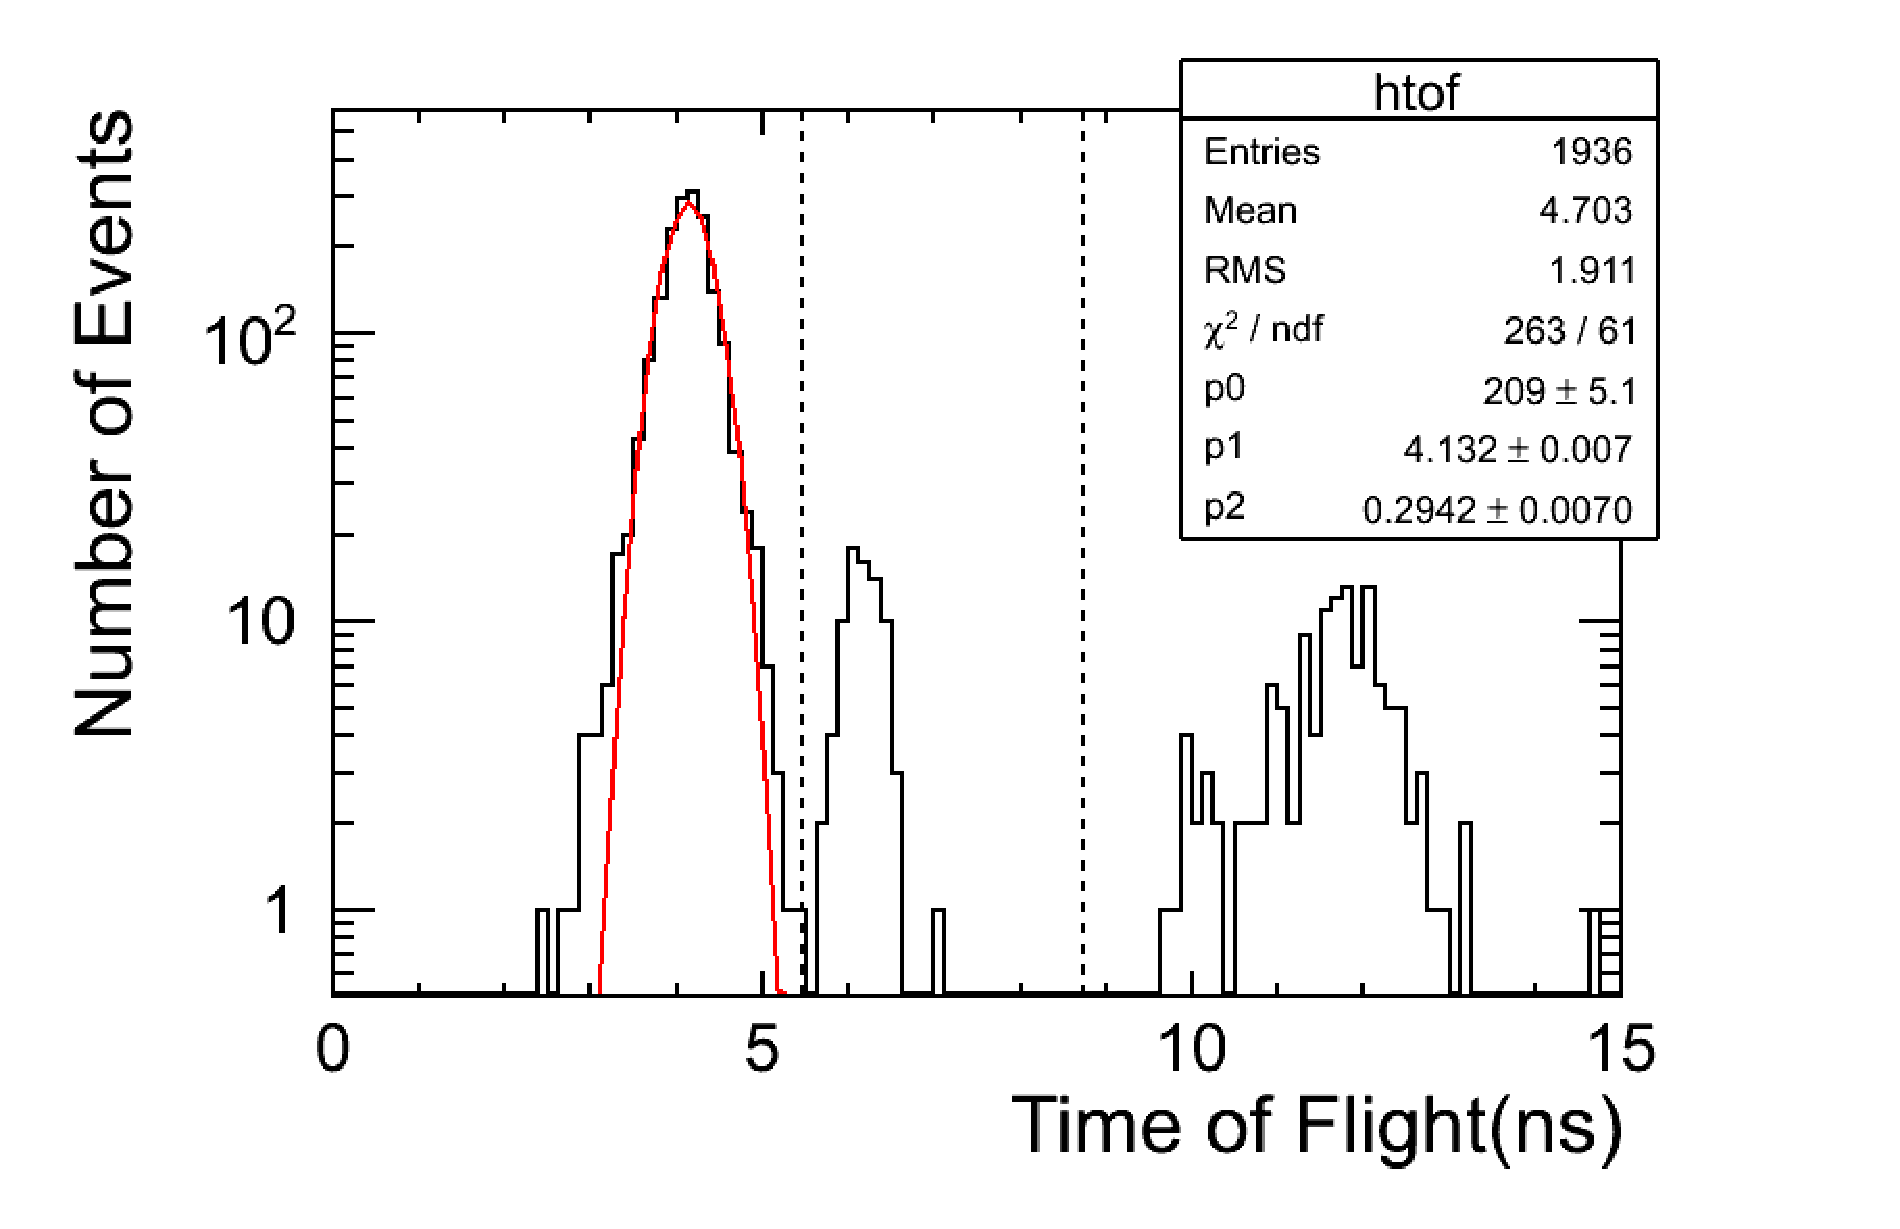
\includegraphics[width=6cm,clip]{fig/TOF.eps}
      \caption{TOF Counter}
      \label{fig:TOF}
    \end{minipage}
    \begin{minipage}{0.5\hsize}
      \centering
      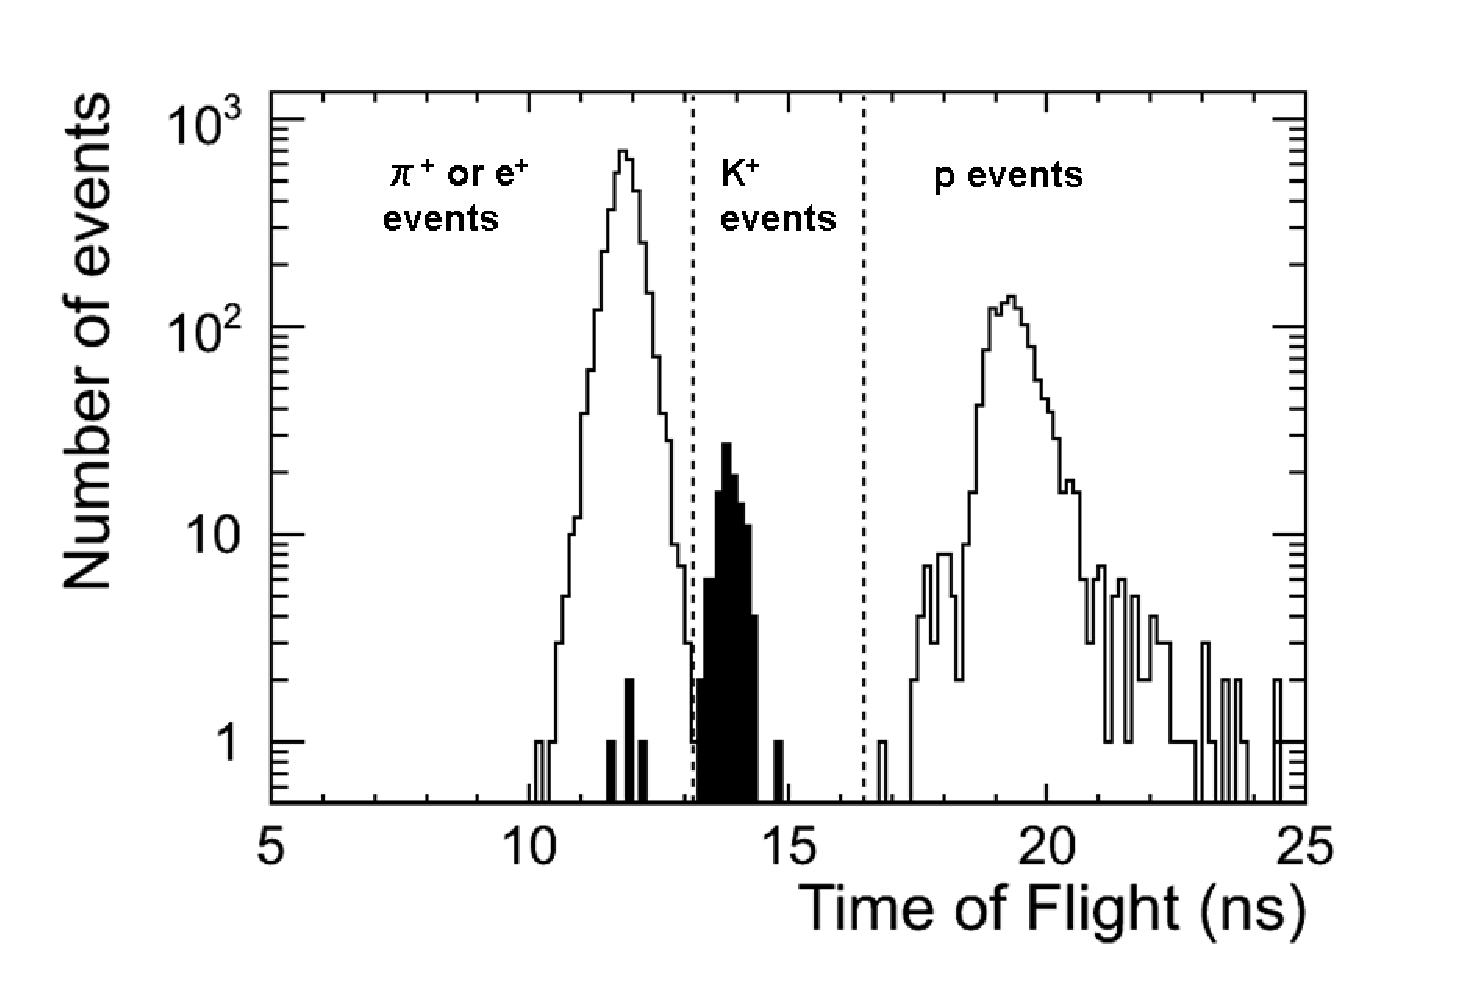
\includegraphics[width=6cm,clip]{fig/TOF_cut.eps}
      \caption{TOF Counter after cut}
      \label{fig:TOF_cut}
    \end{minipage}
  \end{tabular}
\end{figure}

\begin{table}
  \centering
  \caption{Beam components}
  \begin{tabular}[htb]{c|cccc} \hline
               & $e^{+}$ & $\pi$ & $K^{+}$ & $p$ \\ \hline
    Pion run   & 5       & 83    & 3       & 9   \\
    Proton run & 0       & 23    & 0       & 77  \\ 
    Kaon run   & 0       & 0     & 100     & 0   \\ \hline
  \end{tabular}
  \label{tb:beam_component}
\end{table}
